\chapter{How He Built a \$200 Million/Year Security Company}

This lecture offers almost no blackboard mathematics, but it is nevertheless structured by arithmetic, thresholds, deadlines, and causal rules. We begin with the visible endpoint---cars, house, obvious success---only long enough to turn it into a problem. Then the interview proceeds in the order in which the speaker wants us to understand it: first the scale of the outcome, then the mechanism of scale, then the operational rules of focus, savings, pressure, and belief, and finally the deeper interior model by which attention itself is organized.

\section{Status as a Puzzle}

The lecture opens with spectacle and then immediately refuses to stay there. The house and cars are not presented as proof of wisdom; they are presented as the thing to be explained. We are therefore meant to begin with the output and work backward toward the generating mechanism.

The biographical compression matters because it fixes the moral and practical scale of the case. Edwin Arroyave is introduced as someone who came from Colombia, arrived in the United States as a child, lived through poverty and foster care, and assumed household responsibility early. Only after that compression do we get the business anchors: a long career in home security, a nine-figure business, and a very large revenue claim.

The lecture gives us the quantitative frame in a single block:
\begin{equation}
t_{\mathrm{security}} = 25\ \text{years},\qquad
a_{\mathrm{start}} = 21,\qquad
a_{\mathrm{now}} = 46,
\end{equation}
and alongside these,
\begin{equation}
R_{\mathrm{life}} > 600\,\text{million dollars},\qquad
R_{\mathrm{year}} \approx 200\,\text{million dollars}.
\end{equation}

These are interview claims, not audited statements, but they do the work the lecture needs them to do. They tell us that we are not dealing with a small anecdote. We are dealing with a case in which the speaker believes he has found a repeatable operating logic.

\section{Influence, Faith, and Necessity}

Once the host asks how a nine-figure business was scaled, the lecture stops being biographical and becomes operational. The first answer is not technology, not pricing, and not even sales process. It is influence: to build at scale one must attract good people, and good people must believe in the leader and in the dream.

We can summarize the speaker's scaling thesis in the compact form
\begin{equation}
\text{Big dream} + \text{influence}
\Longrightarrow
\text{good people commit}
\Longrightarrow
\text{scale}.
\end{equation}

The important move in the lecture is that this does not remain abstract for long. It is immediately grounded in a concrete memory: the minivan was purchased before the team existed. The action comes before the resources are fully assembled.

\begin{definition}
In the vocabulary of this lecture, faith is not merely assent. It is taking action before one has everything one thinks one needs.
\end{definition}

The speaker then adds a second concept, ``necessity level,'' which is meant to explain why premature commitment can be productive. Once money is spent and the door is shut behind us, dormant effort becomes available. The lecture makes this into a heuristic law:
\begin{equation}
\text{Low stress} \Longrightarrow \text{low performance}.
\end{equation}

We should not read this as a universal scientific law. It is an entrepreneurial rule of thumb. Its force lies in the speaker's claim that pressure, when deliberately chosen, can untap ability that would otherwise remain unused. This is the first major rhythm of the lecture: abstraction, anecdote, operational law.

\section{Focus Before Diversification}

The next question widens from inner drive to business strategy. Should one diversify early, or should one stay concentrated? The answer is strongly sequential. First one builds a dependable core. Only then does one branch outward.

In the lecture's own logic, the rule is
\begin{equation}
\text{Focus first}
\Longrightarrow
\text{bread-and-butter cash flow}
\Longrightarrow
\text{diversification later}.
\end{equation}

The security business is presented as that bread-and-butter engine. Solar appears later, not as a random leap, but as an extension made possible by earlier discipline. The speaker's own comparison makes the point sharply:
\begin{equation}
17\ \text{years in security} \Longrightarrow 40\,\text{million in one year of security},
\qquad
1\ \text{year in solar} \Longrightarrow 40\,\text{million in one year of solar}.
\end{equation}

The second number is not meant to erase the first. It depends on it. The lecture's argument is that what looks like rapid diversification is actually leveraged concentration. One pays the price for a long time in one domain, and then that accumulated discipline, identity, and process travel into another.

\section{Financial Architecture and the First Dream}

The financial advice section is where the lecture becomes explicitly numerical. We are given not just motivation, but partition, reserve, and planning horizon. The first rule is the three-way split of income:
\begin{equation}
I = I_{\mathrm{live}} + I_{\mathrm{tax+sav}} + I_{\mathrm{res}},
\qquad
I_{\mathrm{live}} = I_{\mathrm{tax+sav}} = I_{\mathrm{res}} = \frac{I}{3}.
\end{equation}

Here \(I\) denotes a single incoming check or unit of income. One third is for living, one third for IRS and savings, and one third for a reserve account treated as untouchable. The reserve is psychologically important. The speaker insists that for practical purposes it does not exist; this is how it becomes a real reserve rather than a decorative label.

\begin{figure}
\centering
\begin{tikzpicture}[x=1cm,y=1cm]
\draw (0,0) rectangle (3.3,1.2);
\node at (1.65,0.6) {$I_{\mathrm{live}}=\dfrac{I}{3}$};
\draw (4.1,0) rectangle (7.4,1.2);
\node at (5.75,0.6) {$I_{\mathrm{tax+sav}}=\dfrac{I}{3}$};
\draw (8.2,0) rectangle (11.5,1.2);
\node at (9.85,0.6) {$I_{\mathrm{res}}=\dfrac{I}{3}$};
\draw[->] (5.75,2.2)--(1.65,1.2);
\draw[->] (5.75,2.2)--(5.75,1.2);
\draw[->] (5.75,2.2)--(9.85,1.2);
\node at (5.75,2.55) {$I$};
\end{tikzpicture}
\end{figure}

This schematic is a transcript-based reconstruction of the lecture's three-way allocation rule. Its point is not algebraic sophistication. Its point is that financial discipline is imposed by partition before consumption has a chance to expand.

The lecture then turns from steady rule to a single decisive dream: buying the speaker's mother a house. This is the first place where desire is converted into a numerical blueprint.

\subsection{Question \& Answer}

\paragraph{Question.} How does a dream become a concrete plan rather than a mood?

\paragraph{Answer.} By attaching the dream to numbers, a deadline, and an output rate. The lecture gives all three:
\begin{align}
D &= 12{,}000\ \text{dollars}, &
M &= 1{,}400\ \text{dollars/month}, &
\tau &= 90\ \text{days}, \\
s &\in [8,10]\ \text{sales/week}, &
W &= 12\ \text{weeks}, &
N &= sW \in [96,120]\ \text{sales}.
\end{align}

The worked example is elementary but crucial. Once the dream is translated into \(D\), \(M\), and \(\tau\), the plan is no longer mystical. It becomes a weekly production interval. At the low end,
\begin{equation}
N_{\min} = 8 \times 12 = 96,
\end{equation}
and at the high end,
\begin{equation}
N_{\max} = 10 \times 12 = 120.
\end{equation}

The lecture's force lies in the sequence:
\begin{enumerate}
\item name the dream,
\item read off its immediate numerical constraints,
\item place a date on it,
\item convert the date into a weekly quota,
\item refuse to quit the day before the required result appears.
\end{enumerate}

We should notice how the speaker ties arithmetic to psychology. Late-night sales matter not only because they raise totals, but because they build belief. The plan does not merely organize action; it changes self-perception.

\section{Scarcity, Hoarding, and the Abundance Formula}

After the sponsor interruption, the lecture returns to the main argument by asking what separates the middle class from the wealthy. The answer is framed as a difference in relationship to money. A bad relationship produces hoarding. Hoarding blocks contact with the dream. Without contact, there is little motive to act. Then a setback arrives and consumes the savings that were supposed to create safety in the first place.

That loop can be written schematically as
\begin{equation}
\text{Fear} \Longrightarrow \text{hoarding} \Longrightarrow \text{delay}
\Longrightarrow \text{no real action} \Longrightarrow \text{setback} \Longrightarrow \text{fear}.
\end{equation}

The speaker opposes this with what he calls an abundance formula:
\begin{equation}
\text{Become} \to \text{Act} \to \text{Have}.
\end{equation}

The order is the whole point. The lecture insists that we do not first accumulate safely and then later become the sort of person who acts. We become first. We cultivate hope, faith, and belief first. Then we act before all resources are visible. Only then do we arrive at having.

\begin{figure}
\centering
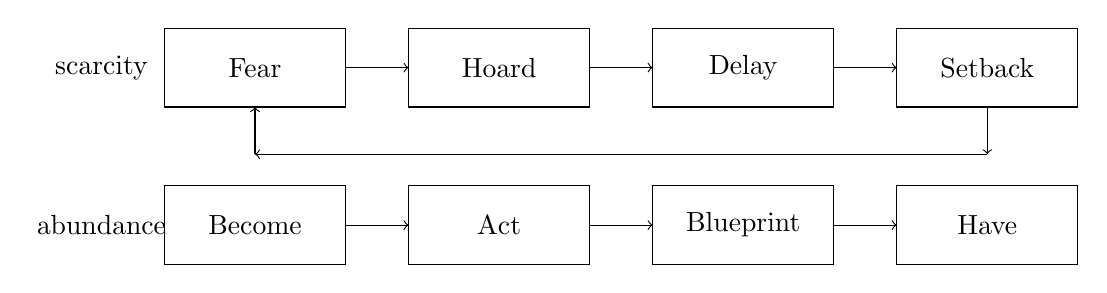
\begin{tikzpicture}[x=1cm,y=1cm]
\node at (-0.8,2.5) {scarcity};
\draw (0,2) rectangle (2.3,3);
\node at (1.15,2.5) {Fear};
\draw (3.1,2) rectangle (5.4,3);
\node at (4.25,2.5) {Hoard};
\draw (6.2,2) rectangle (8.5,3);
\node at (7.35,2.5) {Delay};
\draw (9.3,2) rectangle (11.6,3);
\node at (10.45,2.5) {Setback};
\draw[->] (2.3,2.5)--(3.1,2.5);
\draw[->] (5.4,2.5)--(6.2,2.5);
\draw[->] (8.5,2.5)--(9.3,2.5);
\draw[->] (10.45,2)--(10.45,1.4);
\draw[->] (10.45,1.4)--(1.15,1.4);
\draw[->] (1.15,1.4)--(1.15,2);

\node at (-0.8,0.5) {abundance};
\draw (0,0) rectangle (2.3,1);
\node at (1.15,0.5) {Become};
\draw (3.1,0) rectangle (5.4,1);
\node at (4.25,0.5) {Act};
\draw (6.2,0) rectangle (8.5,1);
\node at (7.35,0.5) {Blueprint};
\draw (9.3,0) rectangle (11.6,1);
\node at (10.45,0.5) {Have};
\draw[->] (2.3,0.5)--(3.1,0.5);
\draw[->] (5.4,0.5)--(6.2,0.5);
\draw[->] (8.5,0.5)--(9.3,0.5);
\end{tikzpicture}
\end{figure}

This diagram is again a transcript-based reconstruction. It adds one intermediate node, ``Blueprint,'' because the lecture repeatedly insists that once action begins, the plan becomes clearer. The blueprint is not fully available in advance. It is generated by movement.

\subsection{Question \& Answer}

\paragraph{Question.} Why does waiting until we have enough money usually leave us stuck?

\paragraph{Answer.} Because in the lecture's logic, waiting is not neutral. Waiting reorganizes the psyche. It makes hoarding feel rational, delays contact with the dream, weakens urgency, and encourages the fantasy that safety must precede motion. The counter-formula is therefore staged:
\begin{align}
\text{Become} &= \text{hope} + \text{faith} + \text{belief}, \\
\text{Act} &= \text{move before resources are complete}, \\
\text{Have} &= \text{the dated objective achieved}.
\end{align}

The lecture then adds one more important clause: after the date is set and the action begins, one should expect a severe test. Just before the blessing comes the punch, the setback, the temptation to revert. The transcript is somewhat garbled at this point, but the operational content is clear enough. The model is not merely linear:
\begin{equation}
\text{Act} \Longrightarrow \text{Test} \Longrightarrow
\begin{cases}
\text{revert to excuses},\\
\text{persist and continue}.
\end{cases}
\end{equation}

This is the place where the lecture's motivational rhetoric is sharpest. The main mathematical content is modest, but the sequencing is strict: date, action, test, persistence, result.

\section{Faith, Happiness, and Attention}

In the final movement the lecture becomes more interior. The speaker wants to explain not only what he did, but how a person keeps the future organized in consciousness long enough to act on it.

First comes the dual definition of faith and fear:
\begin{align}
\text{Faith} &= \text{projection of the best possible future},\\
\text{Fear} &= \text{projection of the worst possible future}.
\end{align}

The lecture's point is that both are future-facing constructions. Neither has happened yet. The difference is not whether we project, but what we project.

Next comes the distinction between pleasure and happiness:
\begin{equation}
\text{Pleasure} = \text{sensation}
\Longrightarrow
\text{pleasure is unstable}.
\end{equation}

The word ``unstable'' matters. Houses, cars, and other exterior factors may produce pleasure, but the lecture argues that they do not by themselves produce durable happiness. Happiness is re-centered inside the subject through gratitude and the active conversion of negative experience into positive interpretation. We need not formalize that more aggressively than the lecture does.

Finally the speaker introduces the reticular activating system as a model of selective attention. We should present it cautiously: not as rigorous neuroscience, but as the speaker's explanatory framework for how earlier dreams, promises, and identity claims became actionable.

\begin{equation}
\mathrm{RAS}:\ (\text{dreams},\ \text{self-worth},\ \text{survival})
\longmapsto
\text{conscious attention}.
\end{equation}

\begin{figure}
\centering
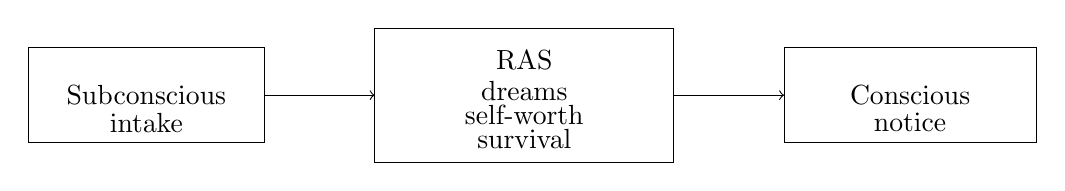
\begin{tikzpicture}[x=1cm,y=1cm]
\draw (0,0.5) rectangle (3,1.7);
\node at (1.5,1.1) {Subconscious};
\node at (1.5,0.75) {intake};

\draw (4.4,0.25) rectangle (8.2,1.95);
\node at (6.3,1.55) {$\mathrm{RAS}$};
\node at (6.3,1.15) {dreams};
\node at (6.3,0.85) {self-worth};
\node at (6.3,0.55) {survival};

\draw (9.6,0.5) rectangle (12.8,1.7);
\node at (11.2,1.1) {Conscious};
\node at (11.2,0.75) {notice};

\draw[->] (3,1.1)--(4.4,1.1);
\draw[->] (8.2,1.1)--(9.6,1.1);
\end{tikzpicture}
\end{figure}

The speaker uses this model to reinterpret his own life. He claims that at a young age he had already fixed three things: a large dream, a rising sense of self-worth, and a survival-grade need to succeed. On this account, opportunity did not merely appear in the world; it became visible because the filtering system had already been trained by desire and promise.

\section{Summary}

The lecture begins with luxury and ends with attention, but its internal order is tighter than that summary suggests. First we are shown scale. Then we are told that scale depends on influence. Then influence is tied to faith, faith to action before resources, action to pressure, pressure to output, output to financial structure, and financial structure to a dated blueprint.

The most concrete formulas in the lecture are simple:
\[
I = \frac{I}{3} + \frac{I}{3} + \frac{I}{3},
\qquad
N = sW \in [96,120],
\qquad
\text{Become} \to \text{Act} \to \text{Have}.
\]
But simplicity here is not weakness. The speaker's claim is that large outcomes come from preserving the order of operations: dream first, partition second, deadline third, action before completion, persistence under test, and only then possession. The final philosophical move---faith against fear, happiness against unstable pleasure, attention filtered by dream and identity---serves as a retrospective explanation of why those earlier operational rules were even usable over a span of decades.